\documentclass[tikz]{standalone}
\usetikzlibrary{matrix}
\begin{document}
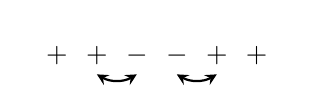
\begin{tikzpicture}
\matrix [%draw=gray,
column sep=0,
%nodes=draw
]
  {
	 \node{$+$}; & \node(a) {$+$}; & \node (b) {$-$}; & \node (c) {$-$}; & \node (d) {$+$}; & \node{$+$}; \\
  };
  \draw [thick,stealth-stealth]  (a.south) to [bend right] (b.south);
  \draw [thick,stealth-stealth]  (c.south) to [bend right] (d.south);
\end{tikzpicture}
\end{document}